\newpage
\section{Ligamentos}

Acá tengo que poner los casos simples y algunos de los casos complejos.

Ver cuando haga ese mini ejercicio para que entreguen, qué quiero poner, como para que tengan algo de variedad.



PG-52 estamos hablando.




%% ver si VPI me presentó un reporte según ASME I.
%% ademas de los ligamentos y las aperturas, ver si menciono algo de los dished heads

%% en cuanto a los desaireadores, poner los tipo de relleno, ver el perry, ver los eductores, ver que estan elevados, ver las toberas, ver el venteo arriba, ver desde el proceso por qué los tengo.

%% ver relleno empaquetados, placas.

%% ASME VIII Div. 1 Ver si VPI me reporto algo de este tacho, incluso lo puedo motrar en clase.

%% Podría llegar a mencionar un tanque flash como otro tanque dentro del alcance de la caldera, y del tanque de enfriamiento de purgas, que si bien tiene una presión mínima, le viene la purga presurizada.

%% Y obviamente, todos los colectores intermedios de caldera, y el colector de vapor sobrecalentado. Todo esto tiene uqe analizarse según código.

%% Se puede estampar el diseño, la fabricación y el montaje. Estampa parcial creo que refiere a los primeros dos.
%% Estampa completa, incluyendo el montaje, es sustantivamente caro si es que tengo que contratar al inspector. Chequear esto, por las dudas


%% bajar el perry novena edicion de libgen en la uba no me deja

\newpage
\section{Derivaciones y compensaciones}

PG-32

Como recomendación de diseño es dable pensar que no vamos a poner los cordones de soldadura, como hace Sobral.

Mandárselo para que le pegue una mirada.












\newpage
\section{Válvulas de seguridad}

Entre los apartados \textbf{PG-67} y \textbf{PG-73}, el código se dedica a establecer los requerimientos para los dispositivos de protección contra la sobrepresión\footnote{Se sobreentiende que la sobrepresión se refiere a un valor por encima de la \textit{MAWP}. Más detalles se presentan más adelante.}.\footnote{El código utiliza la denominación de válvula de alivio de presión (\textit{pressure relief valves}) de manera general, sin entrar en ninguna distinción con la denominación de válvula de seguridad (\textit{pressure safety valve}).} %Es importante destacar que la sección I del código no brinda herramientas para dimensionar los dispositivos de alivio de presión. En lugar de eso, simplemente establece los requerimientos que debe cumplir.

El código genera requerimientos para lo que llama caldera (\textit{boiler}) en el apartado \textbf{PG-67} y para los sobrecalentadores y recalentadores en \textbf{PG-68}. Los requerimientos para los dispositivos de alivio de presión para los economizadores (en los casos en los que apliquen) se encuentran también en el apartado \textbf{PG-67}. La denominación de ''caldera´´ que aquí se usa debe entenderse como la parte del equipo en donde se genera vapor (sea el hogar, sean los tubos pantalla o el haz convectivo si los hubiere).

\subsection{Calderas}

El primer requerimiento que genera el código (en el apartado \textbf{PG-67.1}) es que todas las calderas tienen que tener por lo menos una válvula de alivio de presión. Más aún: las calderas de tubos lisos/desnudos (\textit{bare tubes}), es decir, sin la superficie extendida generada por las aletas, cuya superficie calefactora supere los $A=\SI{47}{m^2}$ deben tener, por lo menos, dos válvulas de alivio de presión. Cuando la superficie calefactora se logra con tubos aletados, el requerimiento de contar con al menos dos válvulas de seguridad se indica para calderas cuya máxima generación de vapor de diseño (establecida por el fabricante) supere $G=\SI{1800}{kg/h}$. Esto es porque la superficie extendida se utiliza con fuentes térmicas de bajo nivel, por lo que puede haber diseños con temperarturas bajas, mucha superficie calefactora y poca generación de vapor para los que el requerimiento de dos válvulas por lo menos es demasiado estricto.

El segundo requerimiento es sobre la capacidad del conjunto de válvulas y sobre el set\footnote{Algunas denominaciones comunes son: timbre, tarado de la válvula, punto de disparo.} de cada una de ellas. Esto es: el punto en el que se inicia la apertura.

El código requiere en el apartado \textbf{PG-67.2.1} que la capacidad de descarga, de alivio (\textit{relieveng capacity}), combinada entre todas las válvulas, sea equivalente a todo el caudal de vapor que puede generar la caldera para todos sus combustibles y de acuerdo con su sistema de combustión, \textit{cuando la caldera está a la $\mathbf{MAWP}$}. Este es un valor que debe informar el fabricante, y puede ser superior que el caudal generable de diseño (\textit{MCR o maximum continuous rating}), debido a los márgenes con los que se diseña la caldera.\footnote{El código presenta algunas sutilezas más en el apartado \textbf{PG-67.2.1} acerca de la capacidad de descarga de las válvulas. Estas reglas debe tenerse en cuenta para el diseño. En \cite{MacKay_Pillow} se encuentra una explicación acerca de esto.}

Naturalmente, una válvula (que no es otra cosa que un orificio calibrado) chica necesita más presión interna para poder descargar ese caudal de vapor que una más grande. Por otra parte, es esperable que la presión crezca mientras la válvula comienza a actuar y hasta que llegue a su capacidad máxima de descarga, ya que estas no actúan inmediatamente.

Para dar cuenta de esto, el código requiere en el apartado \textbf{PG-67.2} que la presión en el interior de la caldera cuando se descarga al exterior toda la capacidad de generación de vapor no supere el 6\% del mayor valor de set de las válvulas. Y, además, que esta presión no supere el 6\% de la $\mathbf{MAWP}$.

Supongamos como ejemplo que una caldera tiene dos válvulas: una con set de $\SI{95}{bar(g)}$ y otra de $\SI{100}{bar(g)}$. Es decir: la primera comienza a abrir cuando la presión interna supera los $\SI{95}{bar(g)}$, y la segunda cuando se superan los $\SI{100}{bar(g)}$. El código requiere que la capacidad total combinada de descarga sea alcanzable cuando la presión interior sea $\SI{106}{bar(g)}$ (como máximo). Este valor debe ser menor que el 106\% de la $\mathbf{MAWP}$.

Esto no implica necesariamente que la $\mathbf{MAWP}$ sea mayor que todos los valores de set de las válvulas. Podría suceder que fuera menor que alguno. En el ejemplo, si la capacidad de descarga total se lograse en $\SI{102}{bar(g)}$ (es decir: permitiendo sólo un 2\% -menor al 6\% máximo- de incremento de presión para la válvula que abre última), podría darse el valor $MAWP=\SI{95}{bar(g)}$. 

En el apartado \textbf{PG-67.2}

Cabe recordar aquí que el código requiere que cualquier presión operativa, permanente o transitoria, no debe superar la $\mathbf{MAWP}$, y que el uso de los dispositivos de alivio es únicamente para situaciones imprevistas.



% poner el dimensionamiento. Poner algun ejemplo. Poner formula. Pensar en que puedan calcular.
% poner eso del 3%
% poner que hay requerimientos sobre el sobrecalentador y sobre el economizador
% hablar de las imagenes que elegi
% aclarar que en la seccion IV I VIII y API son todos requerimientos distintos
% poner en la bibliografia los apuntes que me gusten, y poner el codigo seccion XIII
% Si no pongo mucho más sobre sobrecalentadores y economizadores, borrar la subseccion y dejar solo la seccion










% sobre el dimensionamiento, esta 9764, ahi esta la formula, la tabla para Ksh esta en ASME I. ASME I refiere a ASME XIII, segun interpreto, hay un KD que tiene dar el fabricante (ensayado). Con eso se dimensionan.

% esta libro es una excelente guia y lo explica perfecto
%The Safety Relief Valve
%Handbook
%%Design and Use of Process Safety
%Valves to ASME and International
%Codes and Standards
%Marc Hellemans

%ponerlo en la bibliografia.
% Con esto damos una idea del dimensionamiento.

% Buscar Ksh en el codigo ASME I
% Poner ASME XIII en la bibliografia.

% poner que hay diferencias entre API 520 y ASME VIII. No entraremos en detalles, pero hay diferencias.

% KD es ese coeficiente de descarga, es el que es entre teorico y ensayado, real


 % creo que no interprete bien lo del set, creo que peude ir mas del 6%.

 %Pressure relief valve
%%engineering handbook
%Anderson Greenwood, Crosby And VAreC produCts | Technical publicaTion no. Tp-V300

%de emerson, tiene ejemplos de calculo

%El "simmer" es una apertura gradual y parcial de la válvula antes de alcanzar la presión de ajuste.
%El "popping" es la apertura completa y repentina de la válvula cuando se alcanza la presión de ajuste.

%chatter

%blodown, que es la presio nde reset
%luego, el drain de la descarga

% conservar estas notas aqui, no borrarlas

% K = 0.9 x Kd

% ahi lo dice 9.7.6.5

% ver cómo citar la bibliografía.






















%chequear el libro de mckay, a ver qué dice más lo de psvs que baje
% en principio la formula no la voy a poner.
% Tratar de hacer un resumen, aunque voy a tener que leer un poquito sobre esto.
% poner en la bibliografia algo de calculo de las PSVs, lo que me baje
% el de mckay lo explica bien, leerlo y robar data de alli.

% ALGO IMPORANTE ES QUE EL CODIGO ASME I NO DICE COMO DIMENSIONAR LA VALVULA, SOLAMENTE LE IMPONE REQUERIMIENTOS


% https://annas-archive.org/md5/f922373c882e21d6952f62544dd74d06

% https://annas-archive.org/md5/106071f4ddefd408f383586cd2bd54dd

% https://annas-archive.org/md5/d8c268ec7a4e4c53d73fd806f94a3b74


%PG-67.1
%Minimum Number of Pressure Relief Valves Required

%Dbe have two or more pressure relief valves

%Los dispositivos de alivio de presión son las PSV, pressure safety valve, las válvulas de seguridad, coloquialmente.


%PG-67.2
%The total combined relieving capacity for
%each boiler (except as noted in PG-67.2.1.6, PG-67.4,
%and PL-54) shall be such that all the steam that can be
%generated by the boiler is discharged without allowing
%the pressure to rise more than 6\% above the highest

%Acá se completa lo que vimos en la MAWP. No sólo la sobrepresión admisible cuando se están descargando, sino qué caudal deben descargar. Con esto, se pueden dimensionar los dispositivos.

%PG-67.3
%One or more pressure relief valves on the
%%boiler proper shall be set at or below the maximum allow-
%able working pressure (except as noted in PG-67.4). If
%additional valves are used the highest pressure setting
%shall not exceed the maximum allowable working pres-
%sure by more than 3\%. The complete range of pressure
%%settings of all the saturated-steam pressure relief valves
%on a boiler shall not exceed 10\% of the highest pressure to
%%which any valve is set. Pressure setting of pressure relief
%valves on high-temperature water boilers15 may exceed
%this 10\% range. Economizer pressure relief devices
%required by PG-67.2.1.6 shall be set as above using the
%MAWP of the economizer


%Poner una foto de una válvula de seguridad, que se vea el resorte ,el tornillo de calibracion, y una foto en la que se vean en una caldera, tanto en una humo como en el domo.

%Chequear pero creo que tanto el eco como el sobrecalentador o el recalentador deben tener sus propios dispositivos de alivio.

%chequear si si  si tienen que ser dos

\begin{figure}[ht]
    \centerline{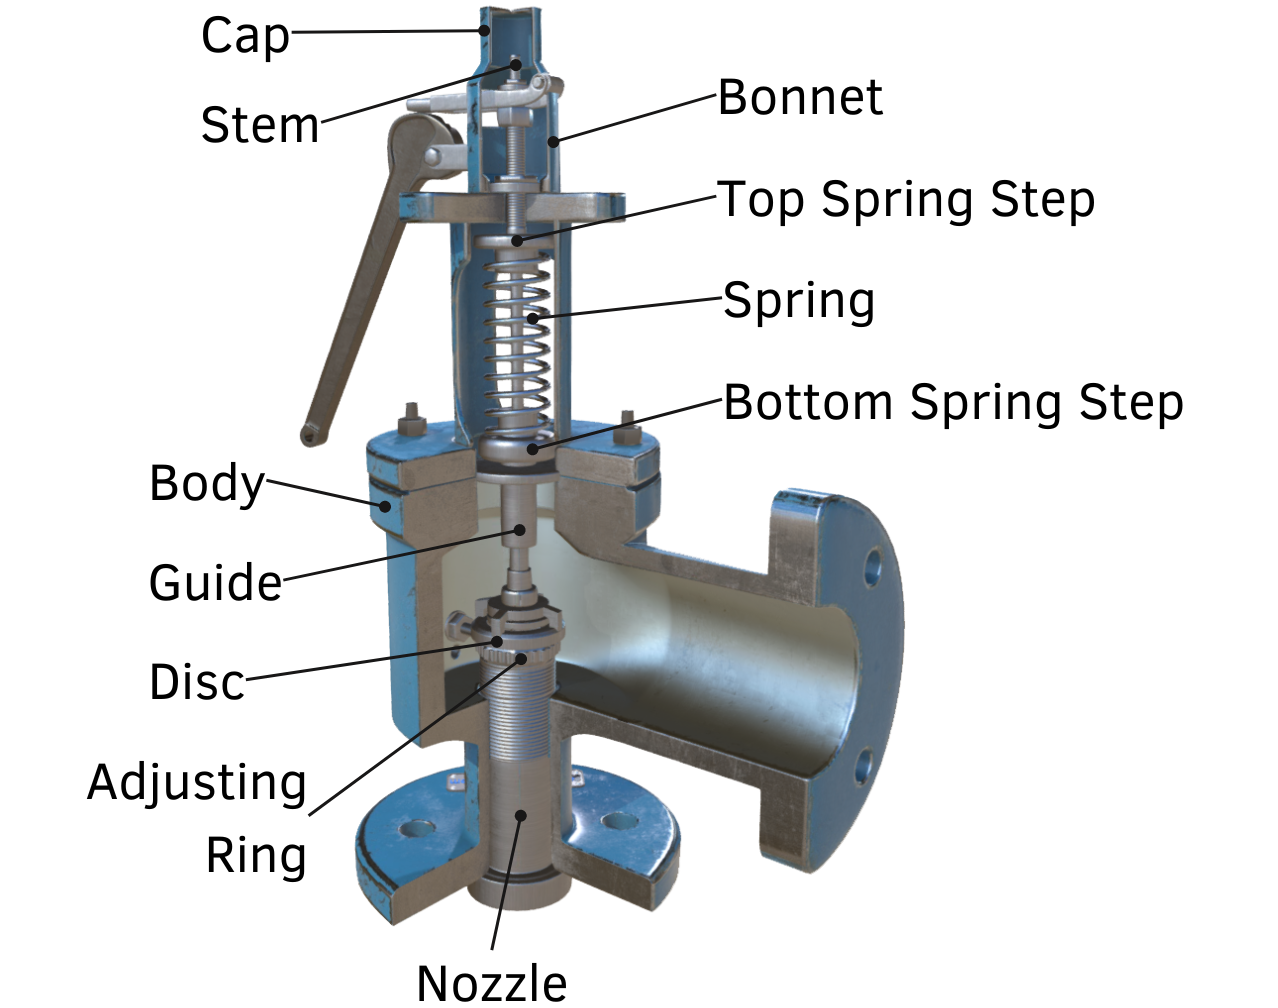
\includegraphics[scale=0.2]{spring_loaded_safety_valve_01.png}}
    \caption{\textit{TBD.}}
    \label{im:spring_loaded_safety_valve_01}
\end{figure}

\begin{figure}[ht]
    \centerline{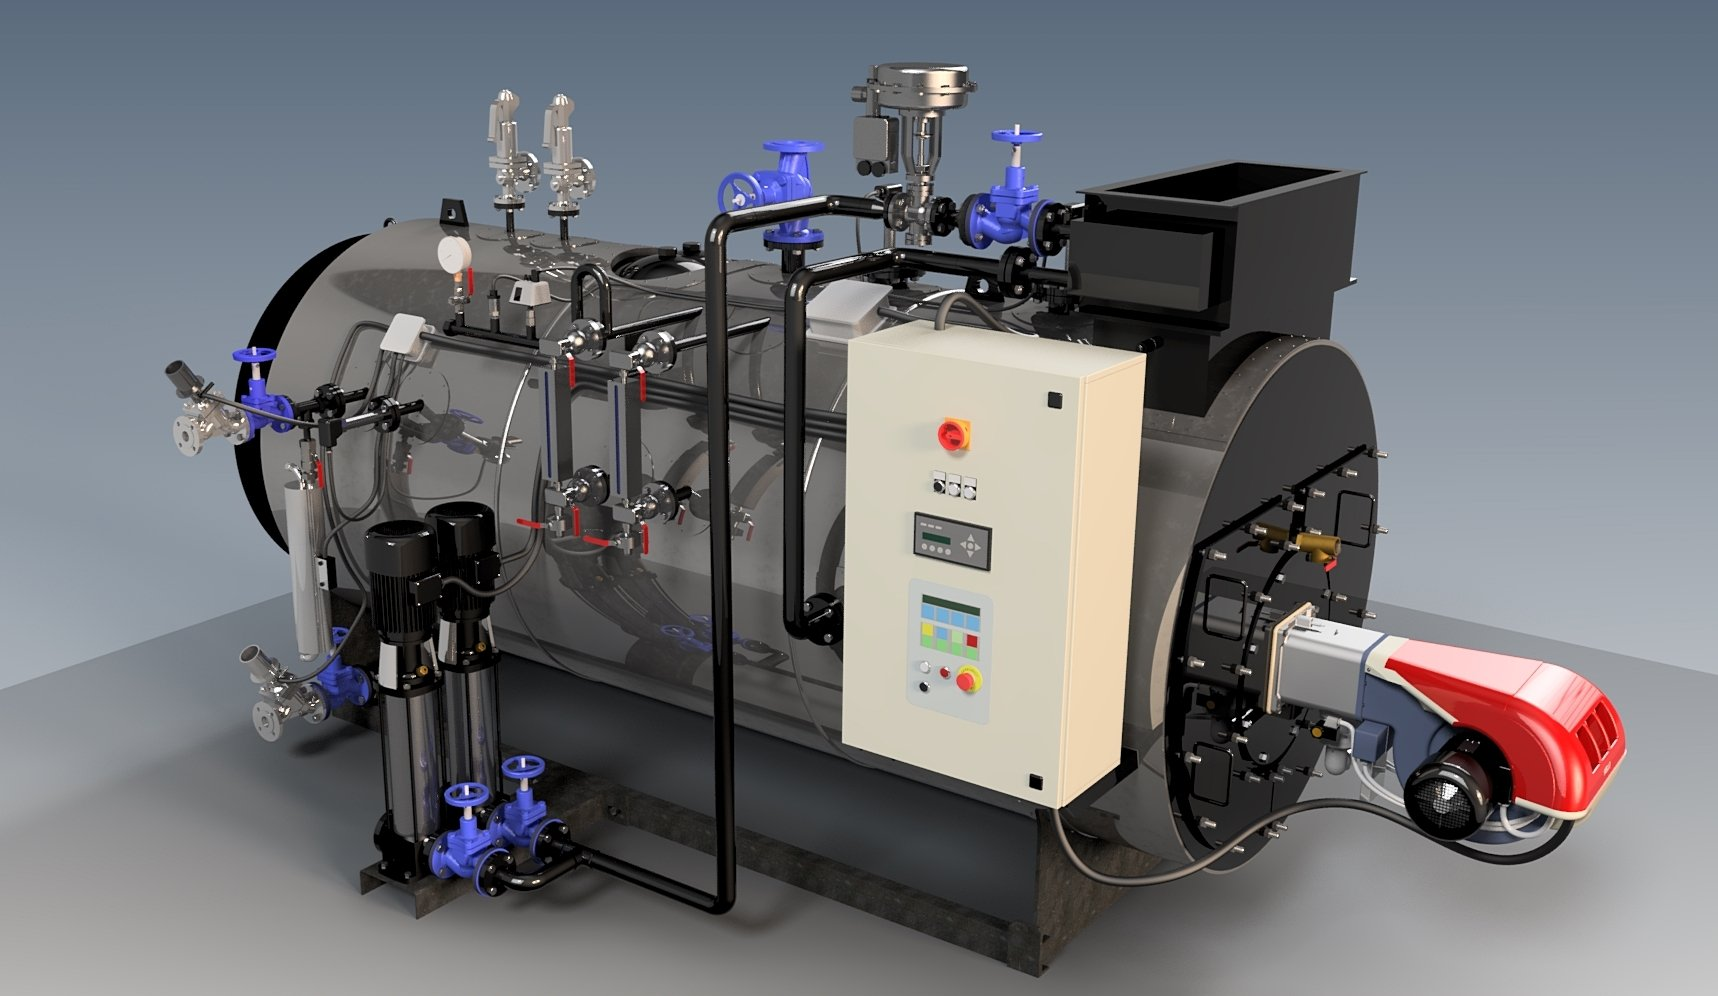
\includegraphics[scale=0.2]{two_psv_firetube_boiler.jpg}}
    \caption{\textit{TBD.}}
    \label{im:two_psv_firetube_boiler}
\end{figure}





\newpage
\section{Comentarios finales y conclusiones}

Poner aca todo lo que dejamos por afuera, o mencionar algunas de las partes.

Concluir algo.








%PAGINA 20 tabla 1A

%linea 45

%resistencia mecanica minima 485 MPa
%fluencia minima 260 MPa
%G10 S1 T2
%Limite maximo de temperartura 454 C

%buscar si tengo algun calculo ferrer de estos
%tiene soldaduras longitudinales y cirfunferenciales

%cabezal de medida distinta a la envueltas
%Ver PG-6, que me admite este material
%considerando que domo va aislado, lo vamos a poner todo a temperatura de saturacion

%apendice de grafitizacion

%asme II non mandatorio A 201 y 202

%mencionar algo de la eficiencia de la soldadura. Medio que pasarlo por alto, la verdad.

%Lo mismo sobre los casquetes, para no marearme yo y no marear a los estudianbtes.

%Sí poner lo de la grafitizacion.






